\chapter{Biological Background}
\chaptermark{Background biologico}



\section{La cellula e la membrana cellulare}
\label{sec:cell}
Le cellule sono le unità fondamentali di tutti gli organismi viventi.
Questi organismi possono essere costituiti da un'unica cellula, detti unicellulari, oppure da più cellule, detti multicellulari.
Per quanto grande e complesso possa essere l'organismo, ogni cellula mantiene sempre la sua individualità e la sua indipendenza.

Benché diverse, le cellule hanno proprietà strutturali comuni.
Il volume interno è definito dal \textbf{citoplasma}, questo contiene una soluzione acquosa in cui sono disciolte una varietà di particelle insolubili, tra cui enzimi, RNA e metaboliti prodotti da varie vie biosintetiche.

Tra le particelle in sospensione nel citoplasma è possibile distinguere vari organelli, ognuno con una diversa funzione.
Tra i principali vi sono i \textbf{ribosomi}, dove avviene la sintesi proteica, il \textbf{reticolo endoplasmatico}, che organizza la sintesi delle proteine e dei lipidi, il \textbf{complesso del golgi}, che modifica e indirizza le proteine alla loro sede finale, i \textbf{lisosomi}, sede preferenziale per reazioni di degradazione, i \textbf{mitocondri}, dove viene prodotta l'energia necessaria alla cellula per il suo funzionamento, e il \textbf{nucleo}, atto a contenere il genoma.\cite{nelsonprincipi}

\begin{figure}[h]
\begin{center}
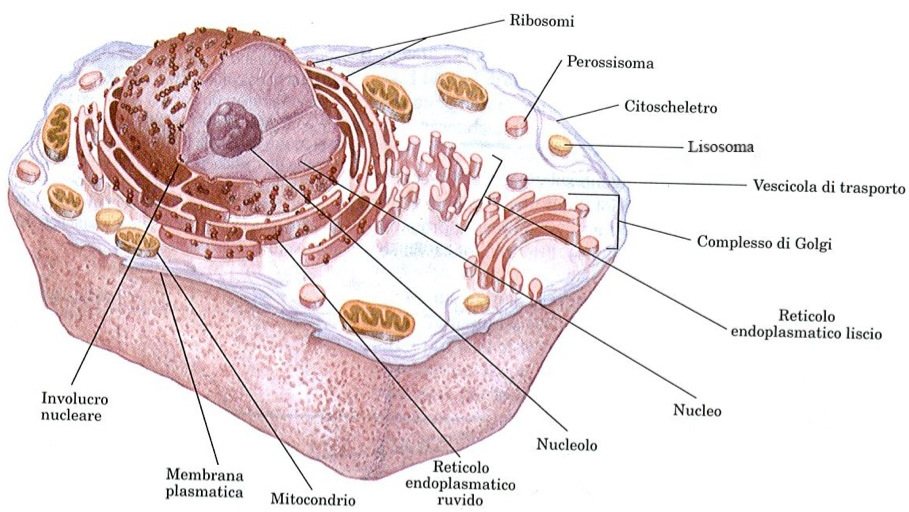
\includegraphics[scale=0.4]{../imgs/cell.png}
\caption[La cellula]{Disegno schematico di una cellula. (Immagine adattata da \cite{nelsonprincipi})}
\label{Fig:cell}
\end{center}
\end{figure}

Ciò che separa la cellula dall'ambiente esterno è definito \textbf{membrana plasmatica}, costituita da un gran numero di lipidi e proteine che sono associate tra loro da un doppio strato idrofobico sottile e flessibile che circonda tutta la cellula e che rappresenta una barriera al passaggio della maggior parte di composti carichi e polari. 
La sua composizione le permette di essere resistente ma flessibile, auto-sigillante e selettivamente permeabile a soluti polari. 
La sua flessibilità, inoltre, consente modificazioni della forma della cellula che hanno luogo durante la crescita e il movimento.

La membrana non è soltanto una barriera passiva, ma contiene anche proteine specializzate che promuovono o catalizzano un gran numero di eventi molecolari.
%Alla superficie delle cellule, i \textbf{trasportatori} spostano molecole organiche specifiche e ioni inorganici attraverso la membrana; i \textbf{recettori} sulla membrana plasmatica sentono i segnali extracellulari convertendoli in modificazioni all'interno della cellula; le \textbf{molecole di adesione} tengono unite cellule vicine. 
%All'interno delle cellule, le membrane sono il supporto per un gran numero di processi cellulari, come la sintesi dei lipidi e di certe proteine, la trasduzione energetica nei mitocondri e nei cloroplasti.
%
%La superficie esterna dei una cellula è in contatto con altre cellule, con il fluido extracellulare e con i suoi soluti, cioè sostanze nutrienti, ormoni, neurotrasmettitori e antigeni. 
Contiene, infatti, una grande varietà di \textbf{trasportatori}, proteine che attraversano la membrana trasportando sostanze nutrienti all'interno e prodotti di scarto all'esterno della cellula. 
Molte proteine sono disposte sulla superficie della cellula (\textbf{recettori di segnali}) e possiedono siti altamente specifici che legano molecole di segnale extracellulari (\textbf{ligandi dei recettori}). 
Quando un ligando esterno si lega al suo recettore specifico, la proteina recettrice trasforma il segnale portato dal ligando in un messaggio intracellulare. 

\begin{figure}[h]
\begin{center}
\includegraphics[scale=0.4]{../imgs/channels.png}
\caption[I canali trans-membrana]{Le tre categorie principali di proteine che fungono da trasportatori attraverso la membrana plasmatica. (Immagine adattata da \cite{nelsonprincipi})}
\label{Fig:channels}
\end{center}
\end{figure}

Per esempio, alcuni recettori di superficie sono associati a \textbf{canali ionici}  che si aprono quando il sito del recettore viene occupato, permettendo l'ingresso di specifici ioni; altri inibiscono o attivano enzimi intracellulari posti sulla superficie interna della membrana.

Qualunque sia il sistema di \textbf{trasduzione del segnale}, i recettori sulla superficie agiscono come degli amplificatori: una singola molecola di ligando che si lega ad un singolo recettore determina un flusso di migliaia di ioni attraverso il canale aperto, oppure la sintesi di migliaia di molecole di un messaggero intracellulare ad opera di un enzima attivato.

Ogni cellula deve recuperare dal suo ambiente circostante il materiale grezzo che le serve per la biosintesi e per la produzione di energia e deve rilasciare sempre nell'ambiente gli scarti del metabolismo.
Questo procedimento viene regolato da due meccanismi l'\textbf{endocitosi} e l'\textbf{esocitosi}.

\begin{figure}[h]
\begin{center}
\includegraphics[scale=0.35]{../imgs/endoeso.png}
\caption[Endocitosi ed Esocitosi]{Rappresentazione schematica dei processi di endocitosi (nella parte sinistra della cellula), ed esocitosi (nella parte destra della cellula).  (Immagine adattata da \cite{nelsonprincipi})}
\label{Fig:endoesocitosi}
\end{center}
\end{figure}

Il primo è un meccanismo che serve a trasportare nel citoplasma i componenti presenti nell'ambiente che circonda la cellula. Durante questo processo una regione della membrana plasmatica si invagina, racchiudendo al suo interno un piccolo volume del fluido esterno. L'invaginazione si richiude poi su se stessa, formando una vescicola rivolta verso l'interno della cellula.
Questa vescicola (l'\textbf{endosoma}) può muoversi dentro la cellula trasportando il suo contenuto a un altro organello circondato da membrana, mediante fusione delle due membrane. L'endosoma serve quindi come estensione della membrana plasmatica, consentendo il contatto tra componenti del mezzo extracellulare e regioni del citoplasma della cellula che non potrebbero altrimenti essere raggiunte per semplice diffusione. 
La \textbf{fagocitosi} è un caso speciale di endocitosi, in cui il materiale trasportato nella cellula (all'interno di un fagosoma) è particolato, come un frammento di una cellula o addirittura un'altra cellula più piccola.
L'inverso dell'endocitosi è l'\textbf{esocitosi} in cui le vescicole si muovono dal citoplasma verso la faccia interna della membrana plasmatica, dove si fondono con essa, rilasciando all'esterno il materiale contenuto. Molte proteine destinate alla secrezione nello spazio extracellulare vengono accumulate in vescicole chiamate granuli di secrezione e rilasciate mediante esocitosi.


\section{DNA e Geni}
\label{sec:dna}
Il DNA è stato isolato per la prima volta dal medico tedesco Friederick Miescher nel 1869, nello stesso importante decennio in cui Darwin pubblicava \textit{L'Origine delle Specie} e Mendel comunicava i suoi risultati alla Società di Storia Naturale di Brùnn. 
La sostanza isolata da Miescher era bianca, zuccherina, leggermente acida e conteneva fosforo.
Poichè era stata trovata soltanto nei nuclei delle cellule, venne chiamata acido nucleico. 
Tale nome fu poi modificato in \textbf{acido desossiribonucleico (DNA)} per distinguere questa sostanza da una simile, l'\textbf{acido ribonucleico (RNA)}. 
Ogni nucleotide è formato da una base azotata, dallo zucchero deossiribosio e da un gruppo fosfato.
Vi sono due tipi di basi azotate: le \textbf{purine}, che presentano una struttura a due anelli e le \textbf{pirimidine} che hanno un solo anello.
Nel DNA vi sono due tipi di purine, l'\textbf{adenina (A)} e la \textbf{guanina (G)} e due tipi di pirimidine, la \textbf{citosina (C)} e la \textbf{timina (T)}, mentre nell'RNA la timina è sostituita dall'\textbf{uracile (U)}.
Così il DNA è costituito da quattro tipi di nucleotidi che differiscono soltanto per tipo di purine o di pirimidine contenenti azoto.

\begin{figure}[h]
\begin{center}
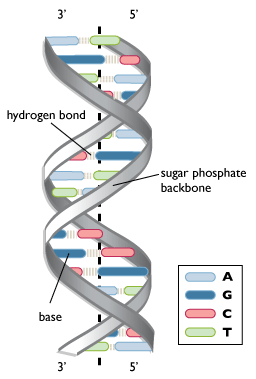
\includegraphics[scale=0.5]{../imgs/dna1.png}
\caption[Il DNA]{Rappresentazione schematica della doppia elica di DNA. Nella legenda sono riportate le quattro basi azotate Adenina, Guanina, Citosina, Timina.}
\label{Fig:dna}
\end{center}
\end{figure}

I primi a scoprire il modello di struttura del DNA (\ref{Fig:dna} a pagina \pageref{Fig:dna}) furono, negli anni '50, lo scienziato americano James Watzon, il fisico francese Francis Crick e la chimica-fisica Rosalind Franklin;  secondo il loro modello la molecola di DNA è un'elica a filamento doppio, dalla forma di una scala a spirale. 
I \textit{pioli} della scala sono costituiti da basi azotate appaiate (una purina si appaia con una pirimidina); A può appaiarsi solo con T e G solo con C, per questo vengono dette \textbf{complementari}. 
Le quattro basi  sono le quattro \textit{lettere} usate per scandire il messaggio genetico.

Un \textbf{gene} è un tratto di DNA che contiene le informazioni per costruire una proteina. I geni sono responsabili dello sviluppo fisico e comportamentale di un organismo e costituiscono le unità portatrici di un carattere ereditario. 
Ogni gene è localizzato in una precisa posizione di un particolare cromosoma. 
Tutte le cellule umane contengono 23 coppie di cromosomi (ad eccezione dei gameti che presentano una singola copia di ciascun cromosoma), ogni cromosoma contiene a sua volta una molecola di DNA con migliaia di geni.

\begin{figure}[h]
\begin{center}
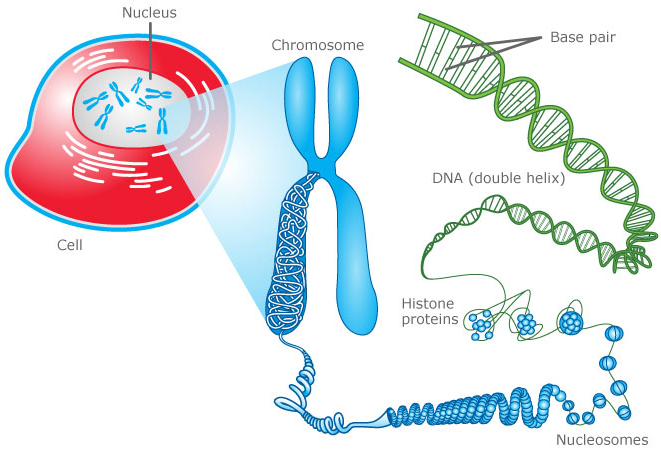
\includegraphics[scale=0.4]{../imgs/dna.png}
\caption[I Cromosomi e il DNA]{Rappresentazione della relazione che intercorre tra DNA e Cromosomi. All'interno del nucleo della cellula sono contenute le coppie di cromosomi, costituiti da cromatina, la cui unità fondamentale è detta nucleosoma, attorno al quale si avvolge il DNA, contenente l'informazione genetica sotto forma di geni.}
\label{Fig:dnachromosome}
\end{center}
\end{figure}

La figura \ref{Fig:dnachromosome} a pagina \pageref{Fig:dnachromosome} aiuta meglio a comprendere la relazione che intercorre tra DNA, gene e cromosoma. 
Gli introni sono regioni non codificanti spesso presenti nei geni eucarioti, eliminate attraverso lo \textit{splicing}: solo gli esoni codificano per le proteine. 
\'E importante sottolineare che finora gli introni erano considerati ''DNA spazzatura'', senza alcuna particolare funzione, ma oggi i ricercatori hanno scoperto che ricoprono un ruolo importante. 
Il dato sorprendente è che esistono sequenze di introni estremamente conservate tra le diverse specie che hanno una funzione nella corretta formazione degli RNA messaggeri. Non è infatti tanto il numero di geni quanto il modo in cui il loro funzionamento è regolato a rendere l'uomo, uomo e il topo, topo. Basti pensare che l'uomo ha circa lo stesso numero di geni del topo.

\section{L'espressione genica}
\label{sec:genica}
La chiave per comprendere i complessi meccanismi della regolazione del metabolismo cellulare consiste nell'interpretare il flusso di informazioni che hanno luogo secondo regole comuni alla maggior parte degli organismi viventi. Le informazioni sono conservate all'interno della molecola del DNA e possono essere sia riprodotte per duplicazione che utilizzate per produrre un vero e proprio messaggio, che ha come obiettivo finale una ben determinata azione chimica. 
L'unità fondamentale dell'ereditarietà, il gene, è un frammento di DNA in grado di codificare un prodotto specifico o, in generale, una o più funzioni correlate. 
Il processo di espressione genica per assemblare la struttura amminoacidica di una proteina avviene in due fasi:
\begin{itemize}
\item \textbf{trascrizione:} un enzima (\textit{RNA polimerasi}) catalizza la sintesi di una molecola di RNA messaggero (mRNA) usando il gene come modello.
\item \textbf{traduzione:} le informazioni contenute nella sequenza dell'\textit{mRNA} determinano la sintesi di uno specifico polipeptide, eseguita dal ribosoma.
\end{itemize}

Volendo apprezzare con maggiore dettaglio il processo di espressione genica, va anzitutto ricordato che la fase di trascrizione ha inizio quando l'enzima RNA polimerasi si lega ad una regione del DNA chiamata \textbf{promotore}. 
Un promotore, tipicamente localizzato in prossimità dei geni, è una regione del DNA in cui le proteine come i fattori di trascrizione possono legare. 
Questi siti contribuiscono all'attivazione della trascrizione delle successive sequenze di geni aumentandone oppure inibendone la trascrizione. 
In prossimità del complesso formato da RNA polimerasi e DNA \textit{promoter}, la doppia elica del DNA si srotola parzialmente e l'enzima può muoversi lungo il filamento modello nella direzione 3'-5'\footnote{3'-5' indica la direzionalità da un estremo all'altro di un singolo filamento di acido nucleico. Il verso opposto, tipicamente del filamento complementare, viene indicato con 5'-3'.}, polimerizzando nella direzione opposta.
Dal momento che il promotore impone alla polimerasi l'orientamento sul DNA e che la polimerizzazione può avvenire in una sola direzione (5'-3'), la polimerasi è obbligata a scegliere come modello uno solo dei due filamenti complementari. 
\'E da notare che non sempre viene selezionato lo stesso filamento di DNA, e non sempre nello stesso punto. Ciò dipende dalla posizione del gene che la polimerasi deve trascrivere.
%Se da un lato deve essere scelto un unico filamento di DNA, dall'altro non è detto che la scelta ricada sempre sullo stesso: ciò dipende dal gene. 
La parte del gene che viene trascritta è detta \textbf{trascritto}, ed è una copia di DNA che dà vita ad una molecola di \textbf{RNA messaggero (mRNA)}.

La sintesi della molecola di mRNA ha termine quando l'enzima RNA polimerasi incontra una sequenza particolare nel filamento di DNA modello che segnala la fine del processo.

L'espressione genica è dunque caratterizzata da un flusso di informazioni che va dal DNA all'RNA, alle proteine. 
Mentre DNA e RNA sono scritti con un alfabeto in base 4, nel caso delle proteine l'alfabeto è in base 20.
Il termine traduzione indica infatti il passaggio da un alfabeto a 4 lettere (le basi azotate degli acidi nucleici) a un alfabeto a 20 lettere (tanti quanti sono gli amminoacidi costitutivi delle proteine presenti in natura).

\section{I \textit{Pathways}}
\label{sec:pathways}
Un \textbf{pathway} è una concatenazione di reazioni che avviene in maniera sequenziale per svolgere una funzione biologica. 
A seconda del tipo di funzione svolta vengono distinte due principali categorie di \textit{pathway}, i pathway di \textbf{trasduzione del segnale} (\textit{signaling pathways}) e i pathway \textbf{metabolici} (\textit{metabolic pathways}).
I \textit{pathway} di trasduzione del segnale servono a processare l'informazione ambientale e a tradurla in una risposta a livello di espressione genica, metabolismo e comportamento.
Mentre i \textit{pathway} metabolici comprendono quelle reazioni che servono per costruire componenti cellulare o per smontarli e produrre energia.

\'E da tenere presente che tutti i \textit{pathways} nella cellula parlano tra di loro, qualunque sia il loro scopo finale. Quindi, bisogna pensare che questa è una suddivisione concettuale necessaria a comprendere meglio determinate funzioni cellulari.

\subsection{Vie di trasduzione del segnale - \textit{Signaling pathways}}
\label{sec:signaling}
La comunicazione tra cellule è mediata principalmente attraverso segnali molecolari. 
Alcuni di questi operano su lunghe distanze, comunicando con cellule lontane; altri comunicano solo con gli immediati vicini. 
La maggior parte delle cellule negli organismi multicellulari inviano e ricevono segnali. 
%Questa comunicazione della cellula con il suo ambiente è cruciale per tutte le funzioni di tessuti e organi.
La recezione dipende dalle proteine recettrici, tipicamente situati sulla superficie della cellula, che legano la molecola del segnale.
Il ligando attiva il recettore, che a sua volta attiva uno o più \textit{pathway} di segnalazione intracellulare.\cite{alberts2000molecular}

La segnalazione intracellulare è regolata da una combinazione di molecole di due tipi: grandi e piccole, al fine di trasmettere i segnali ricevuti sulla superficie della cellula verso il suo interno.
La catena di eventi di segnalazione intracellulare risultante altera le proteine effettrici che sono responsabili della modifica del comportamento della cellula. 

\begin{figure}[h]
\begin{center}
\includegraphics[scale=0.3]{../imgs/signaling.jpg}
\caption[Vie di trasduzione del segnale]{Un esempio di pathway di segnalazione cellulare attivato da una molecola di segnale extracellulare. (Immagine adattata da \cite{alberts2000molecular})}
\label{Fig:signaling}
\end{center}
\end{figure}

Le molecole piccole per la segnalazione intracellulare sono chiamate \textit{piccoli mediatori intracellulari}, o \textit{secondi messaggeri} (i \textit{primi messaggeri} sono i segnali extracellulari). 
Sono generati in gran numero in risposta all'attivazione dei recettori e sono spesso diffusi dalla loro sorgente, diffondendo il segnale in altre parti della cellula.
Sia che siano solubili in acqua, sia che siano lipido-solubili, passano il segnale tramite \textit{binding} o alterando la conformazione e il comportamento di proteine di segnalazione o di proteine effettrici.

Le molecole grandi sono le \textit{proteine di segnalazione intracellulare}, che aiutano a trasmettere il segnale nella cellula generando piccoli mediatori cellulari o attivando il successivo segnale o proteina effettrice nel \textit{pathway}.
Queste proteine formano una rete funzionale, in cui ogni proteina aiuta a processare il segnale in uno o più modi.
\begin{enumerate}
\item La proteina può \textit{trasmettere} il segnale al successivo componente di segnalazione nella catena
\item Può fungere da \textit{impalcatura} per portare due o più proteine di segnalazione insieme così che possano interagire più velocemente ed efficientemente.
\item Può \textit{trasdurre} il segnale in una forma differente, che è adatta sia a passare il segnale in avanti che a stimolare una risposta della cellula.
\item Può \textit{amplificare} il segnale che riceve, sia producendo un più grande ammontare di un piccolo mediatore intracellulare  o attivando più copie di una proteina di segnalazione più in basso nel flusso di trasmissione. In questo modo, un piccolo numero di molecole di segnale extracellulare può invocare una grande risposta intracellulare. Quando ci sono più passi di amplificazione in una catena , la catena è spesso chiamata \textbf{cascata del segnale} (\textit{signaling cascade}).
\item Può \textit{diffondere} il segnale da un \textit{pathway} di segnalazione ad un altro, creando ramificazioni nel flusso di segnalazione, così da incrementare la complessità della risposta.
\item Può \textit{ancorare} una o più proteine di segnalazione in un \textit{pathway} ad una particolare struttura della cellula dove le proteine di segnalazione sono richieste.
\item Può \textit{modulare} l'attività di altre proteine di segnalazione e con ciò regolare la forza della segnalazione lungo il \textit{pathway}.
\end{enumerate}

\subsection{Le vie metaboliche - \textit{Metabolic Pathways}}
\label{sec:metabolic}
Il \textbf{metabolismo}, la somma di tutte le trasformazioni chimiche che avvengono in una cellula o in un organismo, avviene attraverso una serie di reazioni catalizzate da enzimi che costituiscono le \textbf{vie metaboliche} (\textit{metabolic pathways}).
Ogni tappa in successione di una di queste vie produce una piccola ma specifica modificazione chimica, di solito la rimozione, il trasferimento o l'aggiunta di uno specifico atomo o di un gruppo funzionale.
In questa successione di tappe, una molecola di precursore viene convertita in un prodotto attraverso una serie di intermedi metabolici chiamati \textbf{metaboliti}.\cite{nelsonprincipi}

Il \textbf{catabolismo} è la fase degradativa del metabolismo, in cui le molecole organiche delle sostanze nutrienti (carboidrati, grassi e proteine) vengono convertite in prodotti finali più semplici. 
Le vie cataboliche rilasciano energia libera, parte della quale viene conservata mediante la formazione di \textit{ATP}\footnote{L'adenosina trifosfato (o ATP) è uno dei reagenti necessari per la sintesi dell'RNA, nonchè è il collegamento chimico fra catabolismo e anabolismo e ne costituisce la corrente energetica.} e di trasportatori di elettroni in forma ridotta; la parte rimanente viene rilasciata sotto forma di calore.
Nell'\textbf{anabolismo}, chiamato anche biosintesi, i precursori semplici vengono uniti tra loro per costruire molecole complesse più grandi, come i lipidi, i polisaccaridi, le proteine e gli acidi nucleici. 
In genere, le reazioni anaboliche hanno bisogno di un rifornimento di energia.

\begin{figure}[h]
\begin{center}
\includegraphics[scale=0.5]{../imgs/metabolismo.jpg}
\caption[Vie Metaboliche]{Rappresentazione schematica delle reazioni coinvolte nel metabolismo.}
\label{Fig:metabolismo}
\end{center}
\end{figure}

Le vie metaboliche possono essere \textbf{lineari} o \textbf{ramificate}, generando prodotti finali diversi a partire da un unico precursore, oppure convertendo diversi materiali di partenza in un singolo prodotto finale. 
In genere le vie cataboliche sono convergenti, mentre le vie anaboliche sono divergenti. 
Vi sono anche vie \textbf{cicliche}: una molecola di partenza della via viene rigenerata in una serie di reazioni che convertono un'altra molecola di partenza in un prodotto finale.

La maggior parte delle cellule e degli organismi hanno un patrimonio di enzimi che è in grado di catalizzare sia la degradazione sia la sintesi di certi composti.
La sintesi e la degradazione simultanea di alcune molecole comporterebbe uno spreco che viene evitato mediante la regolazione separata delle sequenze di reazioni cataboliche e anaboliche: quando una sta operando l'altra è bloccata.
Questo tipo di regolazione non potrebbe avere luogo se le vie anaboliche e cataboliche fossero catalizzate dallo stesso gruppo di enzimi che operano in direzione dell'anabolismo e del catabolismo: l'inibizione di un enzima coinvolto nel catabolismo porterebbe all'inibizione della sequenza di reazioni nella direzione dell'anabolismo. 


%\section{La trascrizione genica tramite \textit{Microarrays}}
%\label{sec:microarrays}
%Tradizionalmente, la ricerca in biologia molecolare si è occupata dello studio intensivo di uno, o pochi geni alla volta.
%Quando i progetti di ricerca cominciarono a identificare un enorme numero di geni, si cominciarono a sviluppare i \textbf{microarrays}, tecnologie in grado di permettere un'analisi in parallelo dell'espressione di migliaia di geni.
%
%Il tipo di \textit{microarray} dipende dal materiale posizionato sul vetrino; se DNA si parla di \textit{DNA microarray}, nel caso di RNA, viene detto \textit{RNA microarray}, infine, se con tessuto, prende il nome di \textit{tissue microarray}.
%
%Poichè i campioni sono posizionati in modo ordinato, è sempre possibile risalire al gene mappato su una particolare area del vetrino.
%
%Quello più utilizzato è il \textit{DNA microarray} (detto anche \textit{gene chip, DNA chip o biochip}) che è costituito da una serie di sonde (\textit{probes}) di DNA attaccate in maniera ordinata ad una superficie solida come vetro, plastica o silicone.
%Ogni sonda di DNA è a singola elica e rappresenta parte della sequenza di un gene. Nel loro insieme tutte le sonde, di un DNA chip, rappresentano tutti o la maggior parte dei geni di un organismo.
%A seconda della differente tecnologia di produzione dell'array:
%\begin{itemize}
%\item il DNA è posizionato, o sintetizzato direttamente sul supporto.
%\item Le caratteristiche possono essere approssimativamente circolari o rettangolari.
%\item Permettono esperimenti ad un colore o a due colori.
%\end{itemize}
%
%
%Un tipico esperimento tramite \textit{microarray} si sviluppa tramite frammenti di RNA proveniente da una popolazione di cellule precedentemente trattate (a seconda dell'esperimento condotto), i quali vengono versati sul \textit{DNA microarray}, la complementarietà fa in modo che due frammenti possano ibridare, ovvero formare una doppia elica. 
%A questo punto, lavati via i frammenti che non hanno legato, è possibile contare il numero di doppie eliche che si sono formate, risalendo quindi ai livelli di espressione dei geni nella popolazione di cellule.
%
%Tale operazione (detta di scansione) produce in output le immagini grezze delle ibridazioni e un insieme di dati grezzi ricavati direttamente delle immagini. Su questi dati grezzi si effettuano operazioni di normalizzazione al fine di rendere i dati confrontabili tra loro, ottenendo in genere una matrice con i livelli di espressione di ogni \textit{probeset}.
%
%Esistono diversi tipi di \textit{microarray}, solitamente identificati tramite il nome del produttore. I più diffusi sono Affymetrix, Illumina e Agilent. 
%Nel paragrafo successivo verranno descritti brevemente gli array Affymetrix, utilizzati anche dal database \textit{Connectivity Map (CMap)}.
%
%\subsection{I Microarray Affymetrix}
%\label{sec:affymetrix}
%\textit{Affimetrix} utilizza attrezzature simili a quelle impiegate nella realizzazione dei chip di silicio per computer, consentendo di avere una produzione massiva ad un costo ragionevole.
%Così come i chip per computer sono fatti utilizzando maschere che controllano il processo di deposizione e rimozione del silicio dalla superficie del chip, analogamente Affimetrix usa maschere di controllo della sintesi dei campioni sul \textit{microarray}.
%Il risultato è la produzione di alcune centinaia di migliaia di campioni differenti, ciascuno dei quali presente in milioni di copie sul vetrino.\cite{wit2004micro}
%
%\begin{figure}[h]
%\begin{center}
%\includegraphics[scale=0.4]{../imgs/affymetrix.jpg}
%\caption[Microarray Affymetrix]{Un esempio di \textit{Gene Chip} della \textit{Affymetrix}. (Immagine adattata da \cite{wit2004micro})}
%\label{Fig:affy}
%\end{center}
%\end{figure}
%
%Una caratteristica principale dei \textit{microarray Affimetrix} è la misura di un dato trascritto tramite un insieme di \textit{probe} costituiti da 25 basi che varia la sua sequenza di composizione.
%Un insieme di 11 \textit{probe} va a costituire un \textit{probeset}, che lega un singolo trascritto ad una differente posizione lungo la sequenza in analisi. Tendenzialmente, \textit{Affimetrix} contiene decine di migliaia di differenti \textit{probeset}.
%
%Per le analisi di espressione sono utilizzati gruppi di almeno 40 \textit{probe} per gene; \textit{Affymetrix} ha selezionato, per ogni gene, una regione con la minor omologia con altri geni.
%A partire da questa regione sono stati selezionati probe rappresentativi per il \textit{perfect match} (PM), cioè della perfetta complementarità con l'RNA bersaglio, e nucleotidi identici ai precedenti tranne che per la loro base centrale, chiamati \textit{mismatch} (MM), utili a rilevare i segnali non specifici e il segnale in sottofondo catturato da un \textit{probe} PM.
%L'idea è di poter sottrarre l'intensità dell'MM dal PM corrispondente. 
%Un probe PM con il suo corrispondente probe MM viene chiamato \textit{probe pair}.
%
%L'ibridazione di ogni probe con il suo complementare dipende dalla sequenza specifica; poiché si è interessati alla misura del cambiamento di espressione di un gene è necessario ottenere un dato cumulativo da tutte le sonde che identificano quel gene. 
%Questo dato viene calcolato tramite una media della differenza fra le sonde PM e MM dello stesso gene:
%$$AvgDiff=\frac{\sum_{N}(PM-MM)}{N}$$
%dove \textit{N} è il numero di sequenze specifiche che identificano il gene.
%Se il numero che si ottiene da questo calcolo è negativo o molto piccolo significa che il DNA bersaglio è assente o che si è verificata un'ibridazione non specifica.
%%
%%Le fasi di un esperimento di analisi dell'espressione genica che fa uso di \textit{microarray Affymetrix} sono:
%%\begin{itemize}
%%\item Estrazione dell'RNA totale dal campione;
%%\item Separazione del'mRNA dall'RNA totale utilizzando colonnine con code di poly-T;
%%\item Conversione dell'mRNA in cDNA utilizzando la trascrittasi inversa e i primer poly-T;
%%\item Amplificazione del cDNA utilizzando T7 RNA polimerasi in presenza di biotina-UTP e biotina-CTP in modo da ottenere da 50 a 100 copie di cDNA marcato;
%%\item Incubazione del cDNA a 94°C in un buffer di frammentazione per produrre frammenti di lunghezza tra 35 e 200 nucleotidi;
%%\item Ibridazione sul chip e successivi lavaggi;
%%\item Marcatura del cDNA ibridato con Streptavin-Phycoerythrin e successivi lavaggi;
%%\item Acquisizione dell'immagine del chip con scanner laser;
%%\item Analisi dell'immagine per l'estrapolazione dei dati.
%%\end{itemize}
%
%\section{Il drug discovery computazionale}
%\label{sec:dd}
%L'avanzare delle tecnologie come i Microarray ha ha dato la possibilità di poter effettuare test sperimentali di farmaci in vitro, in modo da capire su quali geni o porzioni di DNA vanno ad agire maggiormente.
%
%Tipicamente un nuovo medicinale impiega dai 10 ai 20 anni per essere sviluppato, e molti di questi non riescono ad arrivare sul mercato, con considerevole dispendio economico da parte delle industrie produttrici.
%
%Il processo di produzione di un farmaco è diviso in quattro fasi principali che possono essere riassunte sommariamente come:
%\begin{itemize}
%\item \textbf{Scoperta:} dopo che una malattia o una condizione patologica di interesse è stata identificata, le proteine responsabili sono isolate e caratterizzate (ad esempio, identificando i cambiamenti causali genetici);  poi un \textit{farmacoforo}\footnote{Un \textit{farmacoforo} è la più piccola unità strutturale della molecola di un farmaco, responsabile della sua attività biologica.} è identificato sulla base di queste proteine;
%tipicamente questo viene fatto cercando composti che interagiscono con le proteine \textit{target} usando grandi librerie di composti.
%
%\item \textbf{Sviluppo:} l'obiettivo di questa fase è sintetizzare composti più avanzati, nuovi analoghi con potenza accresciuta e ridotta attività specifica; questa ottimizzazione è compiuta tramite modifiche chimiche del \textit{farmacoforo} (chiamato anche \textit{hit structure}), con modifiche scelte tramite analisi combinata di struttura e attività;
%
%\item \textbf{Sperimentazione clinica:} può variare in dimensione da un singolo centro in un paese, a sperimentazioni in più centri in più paesi. \'E tipicamente divisa in tre fasi principali
%\begin{itemize}
%\item \textbf{Fase I:} a seconda del tipo di prodotto e del livello di sviluppo, gli investigatori coinvolgono volontari sani, e pazienti in piccoli studi pilota.
%\item \textbf{Fase II:} successivamente i test vengono seguiti da studi su più larga scala, su pazienti che spesso confrontano il nuovo prodotto con il trattamento correntemente prescritto.
%\item \textbf{Fase III:} quando vengono ottenuti dati positivi sulla sicurezza e sull'efficacia, il numero di pazienti viene tipicamente incrementato, passando allo \textit{step} successivo.
%\end{itemize}
%
%\item \textbf{Commercializzazione:} il processo pubblicitario e di promozione della vendita del nuovo medicinale approvato.
%\end{itemize}
%
%\begin{figure}[h]
%\begin{center}
%\includegraphics[scale=0.6]{../imgs/ddpipe.jpg}
%\caption[Passi principali di un farmaco]{In questa figura è rappresentato il complesso percorso che un farmaco deve intraprendere per poter essere commercializzato.}
%\label{Fig:drugdisc}
%\end{center}
%\end{figure}
%
%
%I metodi computazionali possono essere usati per predire o simulare se un particolare composto interagisce con una data proteina \textit{target}.
%Inoltre, possono essere usati come assistenti in fase di costruzione riguardo proprietà chimiche desiderabili durante la fase di sviluppo del medicinale e aiutare a rifinire e modificare i medicinali candidati.
%Infine, i metodi computazionali possono essere usati anche per automatizzare compiti ripetitivi come la ricerca in grandi database di composti.
%
%I maggiori vantaggi confrontati a esperimenti di laboratorio sono la diminuzione dei costi.
%\'E possibile, infatti, condurre indagini su composti che non sono stati ancora sintetizzati, selezionandone un insieme per indagini reali in un grande spazio di ricerca in cui il numero di possibili molecole virtuali è più grande del numero reale.
%
%\subsection{L'analisi di reti aiuta a capire il modo di azione di un farmaco}
%\label{sec:moa}
%%
%%Le reti biologiche possono contribuire a capire gli effetti di farmaci usati clinicamente. 
%%Vi sono vari approcci che possono identificare target precedentemente sconosciuti del medicinale e le vie metaboliche che sono affette dal medicinale.
%%Qeusti possono a loro volta essere usati per chiarire gli effetti di offtarget, eventi ostili o suggerire indicazioni aggiuntive o controindicazioni nell'uso del farmaco.
%%mentre molti farmaci hanno target terapeutici noti, molte altre che sono correntemente usato lavorano tramite meccanismi sconosciuti.
%%Inoltre, anche medicinali con un target conosciuto spesso hanno effetti offtarget.
%%ci sono effetti spesso non desiderabili, di un medicinale che può non essere spiegato attraverso la sua interazione con i suoi target primari.
%%Alcuni studi su reti di farmaci hanno permesso l'identificazione di alcuni target secondari per i farmaci. 
%Una rete è un'astrazione naturale di un insieme di oggetti (nodi) e delle relazioni (archi) che intercorrono tra essi.
%Nodi ed archi in una rete possono rappresentare tipi eterogenei di relazioni, a seconda del fenomeno che viene modellato.
%
%Le reti sono state largamente usate per rappresentare interazioni regolatorie e funzionali tra geni, proteine e metaboliti, mappando interazioni verificate sperimentalmente o predette computazionalmente, come archi tra nodi corrispondenti.
%I dati sperimentali genomici, transcrittomici e proteomici, data la loro larga scala, consentono l'identificazione di migliaia di interazioni in un tempo relativamente breve, anche se il loro significato funzionale non è immediatamente evidente.
%
%Il \textit{drug discovery} basato su reti mira a sfruttare il potere di queste per indagare sull'impatto di piccole molecole su reti molecolari in modo da chiarire i suoi meccanismi di azione e per identificare trattamenti terapeutici innovativi.\cite{iorio2013drugrep}
%Queste metodologie innovative possono essere usate per scoprire gli effetti specifici, le interazioni tra il farmaco e il substrato, in modo da aiutare il processo di \textit{drug discovery} durante la fase di ottimizzazione, gli effetti aspecifici, interazioni impreviste tra medicinale e substrato, e gli effetti indiretti, dovuti a segnali di propagazione dopo l'interazione diretta tra il farmaco e il substrato, così facendo aiutano nell'identificazione di nuove opportunità terapeutiche per il \textit{drug repositioning}, ovvero l'applicazione di farmaci conosciuti in nuove applicazioni. 
%Questo processo può riposizionare un farmaco che è già in fase III di sperimentazione clinica, o anche trovare una nuova applicazione per un farmaco che ha superato solo la fase I, per cui si sa che non è nocivo ma non si è riusciti a dimostrare la sua implicazione farmacologica.
%
%L'utilizzo di reti di geni può essere largamente definito come un insieme di nodi rappresentanti geni, ed un insieme di archi tra i geni interagenti ad un livello regolatorio o funzionale.
%Queste connessioni non sono necessariamente di natura fisica, come nel caso di reti di proteine, ma possono rappresentare dipendenze statistiche indiretta tra i geni. 
%Gli archi sono tendenzialmente ricavati da \textit{profili di espressione genica} attraverso analisi computazionali, tendenzialmente tramite \textit{microarray}, oppure usando approcci basati sulla letteratura esistente, senza l'uso di alcun dato sperimentale.
%
%A partire dai profili di espressione genica ricavati da trattamenti di farmaci si possono inferire reti di farmaci. Queste reti descrivono le similarità tra farmaci, come risposte trascrizionali simili o similarità basata su reazioni avverse.
